\documentclass[10pt]{article}\usepackage[margin=.65in]{geometry}\usepackage[T1]{fontenc}\usepackage{graphicx}\setlength{\parindent}{0pt}\setlength{\parskip}{6pt}\sloppy\begin{document}{\large Exact base image layer inspection}\par Read-only inspection on 2026-11-02 verified the exact base image configuration digest and all 10 uncompressed layer digests. The parser visited 19,600 layer headers. In these image layers, /opt and /opt/isolab have explicit directory metadata: mode 0755, UID 0, GID 0. The proposed /fixtures and /qualification paths and their placeholder destinations are absent from every layer. No relevant whiteout or conflicting ancestor type was observed.\par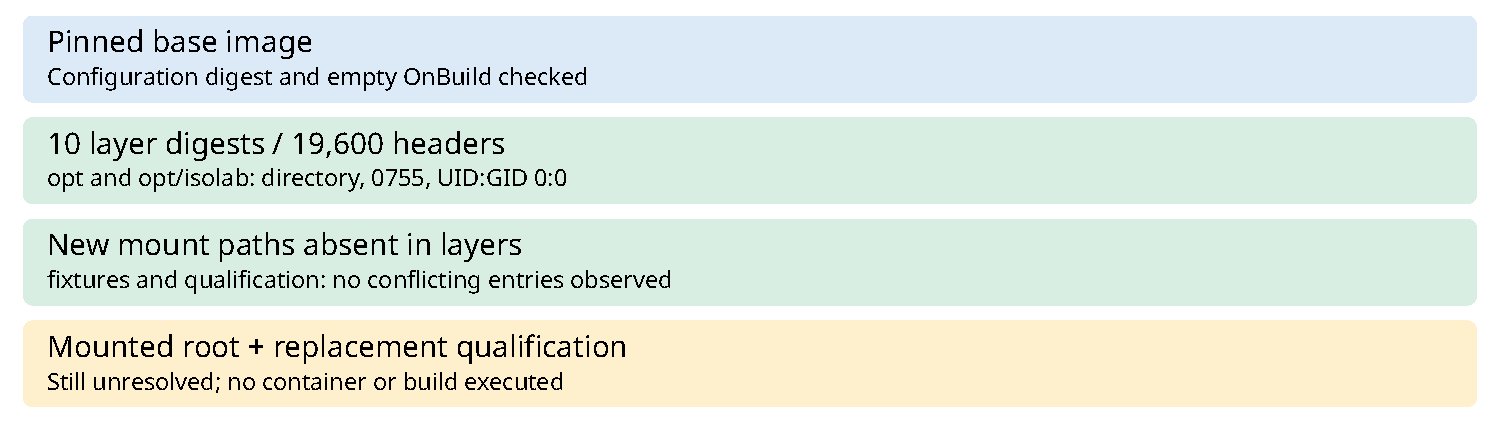
\includegraphics[width=\linewidth]{diagram.pdf}\par Method and identity. Docker image inspect confirmed base sha256:347667d6\allowbreak{}ecc9294a\allowbreak{}b7bfcc83\allowbreak{}411fb47f\allowbreak{}7548c8d1\allowbreak{}ca5f7d31\allowbreak{}5cca23fc\allowbreak{}4b115476 with empty OnBuild. A single image-save call wrote a 549,662,208-byte local archive. The reader checked the exported configuration hash against the exact image ID and every layer against its ordered rootfs.diff\_ids before reading metadata. It extracted no filesystem and ran no image command. The archive checksum, local path, per-layer digests, selected headers and source bindings are in the JSON records.

Failure retained. The first capture wrapper exited 1 because the installed Python lacks hashlib.file\_digest. The failure happened after the save subprocess returned and before receipt serialization. The original save exit code is therefore unknown. We did not repeat the save: a compatible streaming hash implementation verified the retained archive, including all 10 expected layer digests. The first script remains preserved beside the corrected script. Byte integrity is established independently of the missing command-status receipt; no successful exit code was invented.

Filesystem boundary. /opt/isolab/recovery and its lib directory are also absent in this base. The root directory has no explicit layer header, so its eventual mounted mode and ownership remain unspecified by this inspection. Image headers do not establish the daemon's mounted root metadata, ACL behavior, or the replacement image's writable-layer diff. The parser flags relevant whiteouts and non-directory selected paths for manual review; it is a scoped inspector, not a general layer-union implementation.

Next construction. The prior packet already staged the exact 19-member build context. This packet adds verified base identities and selected ancestor metadata, with no path conflict observed for the proposed destinations. Root metadata, bounded assembler and qualification admission, and prospective independent review remain required. A replacement image has not been built; Q1 remains historically failed and the strict empty-diff check remains unchanged. Independent reviewer agents currently report usage-limit failures.

Resources and custody. This was one read-only local save with a 90-second command deadline and a 768 MiB output-file limit. No container creation, container start, build, cloud action or scientific trial occurred. Full raw archive custody is local at the receipt path; no durable remote archive upload is claimed. Published metadata and scripts support replay when those pinned image bytes are available. The 1,260-target scope, prior evidence, and planning allowance of 25,200 worker-seconds ending 2026-11-03 06:00 UTC remain unchanged.

Sources and checks. Docker image-save documentation: https://docs.docker.com/reference/cli/docker/image/save/. OCI filesystem-layer specification: https://github.com/opencontainers/image-spec/blob/main/layer.md. These describe saved parent layers, metadata, links and whiteouts; absent headers are not replaced with assumed runtime defaults. The diagram presents observations and unresolved bindings rather than performance measurements. No scientific graph or cost ratio changes.
\end{document}